% +--------------------------------------------------------------------+
% | LaTeX Template                                                     |
% | for K-State Electronic Theses, Dissertations, and Reports          |
% |                                                                    |
% | Comments and guidelines for using the template are shown           |
% | within boxes like this one.                                        |
% |                                                                    |
% | Revised 6/30/06                                                    |
% | 9/14/06: Removed typos                                             |
% +--------------------------------------------------------------------+

% +--------------------------------------------------------------------+
% | Your paper should contain the following sections, except where     |
% | indicated as optional, in the order shown.  Also, all headings     |
% | shown with an asterisk (*) must be centered and in uppercase       |
% | letters:                                                           |
% |                                                                    |
% | Abstract Title Page (doctoral dissertations only)                  |
% | ABSTRACT* (doctoral dissertations only)                            |
% | Title Page                                                         |
% | Copyright Page (Optional - only needed if copyrighting)            |
% | ABSTRACT *                                                         |
% | TABLE OF CONTENTS *                                                |
% | LIST OF FIGURES *                                                  |
% | LIST OF TABLES*                                                    |
% | ACKNOWLEDGMENTS* (Optional)                                        |
% | DEDICATION * (Optional)                                            |
% | PREFACE * (Optional)                                               |
% | Individual Chapters                                                |
% | References and/or bibliography                                     |
% | Appendices (as needed)                                             |
% +--------------------------------------------------------------------+

% +--------------------------------------------------------------------+
% | The LaTex keyword \documentclass selects a particular class to     |
% | associate with the document.  The current documentclass            |
% | {class_diss} generates a Table of Contents that has leading dots   |
% | only on chapter subheadings.  If you prefer a Table of Contents    |
% | that has leading dots for all entries, replace {class_diss}        |
% | with {Mydiss} in the command below.                                |
% |                                                                    |
% +--------------------------------------------------------------------+

\documentclass[final, 12pt,oneside]{class_diss}

% +--------------------------------------------------------------------+
% | The following command sets the bibliography style to American
% | Institute of Physics (AIP).  Other styles are available in the
% | styles directory.  To use a different style, replace "aip" with
% | the filename of the style you want to use.
% +--------------------------------------------------------------------+

\bibliographystyle{styles/plain}

\usepackage[utf8]{inputenc}
\usepackage[T1]{fontenc}
%\usepackage[spanish]{babel}
% +--------------------------------------------------------------------+
% | Now, we add in all external packages that we will use throughout   |
% | the document.  You can add other packages as needed.
% +--------------------------------------------------------------------+

%\usepackage{     caption2} % Customize captions a bit more
\usepackage{      amsmath} % American Mathematics Society standards
%\usepackage{      wrapfig} % Wraps text around a figure or table
\usepackage{     graphicx} % Extended graphics package.
%\usepackage{     fancyhdr} % Efficiently handles headers and footers
%\usepackage{       braket} % Bra-Ket notation package
%\usepackage{     mathrsfs} % Specialized Math fonts (Hamiltonian, etc.)
%\usepackage{boxedminipage} % Boxed text can be produced
%\usepackage{     setspace} % Controls line spacing via \begin{space}
\usepackage{algorithm}
\usepackage{algorithmicx}
\usepackage[noend]{algpseudocode}
\usepackage{mathtools}

% +--------------------------------------------------------------------+
% | The color package allows one to select colors for hyperlinking     |
% | (see below).                                                       |
% +--------------------------------------------------------------------+

\usepackage[usenames]{color}
\usepackage[table]{xcolor}

% +--------------------------------------------------------------------+
% | Colors defined for use with this template.                         |
% +--------------------------------------------------------------------+

\definecolor{  Pink}{rgb}{1.0, 0.5, 0.5}
\definecolor{Maroon}{rgb}{0.8, 0.0, 0.0}

% +--------------------------------------------------------------------+
% | In the commands below, we use the 'natbib' package, and specify    |
% | the 'sort&compress' option, which condenses                        |
% | citations from (1,2,3,5,9,10,11) to (1-3,5,9-11).  The 'bibpunct'  |
% | option selects various parameters for how the citation will be     |
% | displayed.  In this case, only the comma (separation between       |
% | citations) and the 's' (superscript) arguments are chosen.  The    |
% | other curly braces deal with how to 'wrap' the citation (using     |
% | parentheses, brackets, etc.) and are not needed for the chosen     |
% | style.                                                             |
% +--------------------------------------------------------------------+

\usepackage[sort&compress]{natbib}
\bibpunct{[}{]}{,}{n}{}{}
\usepackage{hypernat}

% +--------------------------------------------------------------------+
% | Lastly, the hyperref package allows one to hyperlink cross-        |
% | references and figures in a LaTeX document.                        |
% +--------------------------------------------------------------------+

\usepackage[pdftex, plainpages=false, pdfpagelabels]{hyperref}

\hypersetup{
    linktocpage=true,
    colorlinks=true,
    bookmarks=true,
    citecolor=blue,
    urlcolor=red,
    linkcolor=Maroon,
    citebordercolor={1 0 0},
    urlbordercolor={1 0 0},
    linkbordercolor={.7 .8 .8},
    breaklinks=true,
    pdfpagelabels=true,
    }

% +--------------------------------------------------------------------+
% | Page margins are set on 1 inch on all sides.                       |
% +--------------------------------------------------------------------+

\topmargin      = -0.56in
\textheight     =  8.60in
\textwidth      =  6.46in
\oddsidemargin  =  0.02in

% +--------------------------------------------------------------------+
% | Stuff for the gantt diagramm.                                      |
% +--------------------------------------------------------------------+

\usepackage{amsxtra}
\usepackage{amssymb}
\usepackage{amsthm}
\usepackage{latexsym}

\usepackage{amsfonts}
\usepackage{amssymb}
\usepackage{geometry}
\usepackage{tikz}
\usetikzlibrary{calc}
\usepackage{graphicx}
% GanttHeader setups some parameters for the rest of the diagram
% #1 Width of the diagram
% #2 Width of the space reserved for task numbers
% #3 Width of the space reserved for task names
% #4 Number of months in the diagram
% In addition to these parameters, the layout of the diagram is influenced
% by keys defined below, such as y, which changes the vertical scale
\def\GanttHeader#1#2#3#4{%
 \pgfmathparse{(#1-#2-#3)/#4}
 \tikzset{y=7mm, task number/.style={left, font=\bfseries},
     task description/.style={text width=#3,  right, draw=none,
           font=\sffamily, xshift=#2,
           minimum height=2em},
     gantt bar/.style={draw=black, fill=blue!30},
     help lines/.style={draw=black!30, dashed},
     x=\pgfmathresult pt
     }
  \def\totalmonths{#4}
  \node (Header) [task description] at (0,0) {\textbf{\large Tasks}};
  \begin{scope}[shift=($(Header.south east)$)]
    \foreach \x in {1,...,#4}
      \node[above] at (\x,0) {\footnotesize\x};
 \end{scope}
}

% This macro adds a task to the diagram
% #1 Number of the task
% #2 Task's name
% #3 Starting date of the task (month's number, can be non-integer)
% #4 Task's duration in months (can be non-integer)
\def\Task#1#2#3#4{%
\node[task number] at ($(Header.west) + (0, -#1)$) {#1};
\node[task description] at (0,-#1) {#2};
\begin{scope}[shift=($(Header.south east)$)]
  \draw (0,-#1) rectangle +(\totalmonths, 1);
  \foreach \x in {1,...,\totalmonths}
    \draw[help lines] (\x,-#1) -- +(0,1);
  \filldraw[gantt bar] ($(#3, -#1+0.2)$) rectangle +(#4,0.6);
  \coordinate (#1a) at (#3,-#1+0.5);
  \coordinate (#1b) at (#3+#4,-#1+0.5);
\end{scope}
}

\newcommand\arrowwhereboxesoverlap[3][]{%
  % #1: arrow style
  % #2: number of first task
  % #3: number of second task
  \path (#2b) ++(0.2,-0.5) coordinate (tmpa);
  \path (#3a) ++(-0.2,0) coordinate (tmpb);
  \draw [#1] (#2b) -| (tmpa) -| (tmpb) -- (#3a);
  }


% +--------------------------------------------------------------------+
% | Stuff for flowcharts.                                              |
% +--------------------------------------------------------------------+
\usetikzlibrary{shapes.geometric, arrows}

\tikzstyle{startstop} = [rectangle, rounded corners, minimum width=3cm, minimum height=1cm,text centered, draw=black]
\tikzstyle{io} = [trapezium, trapezium left angle=70, trapezium right angle=110, minimum width=3cm, minimum height=1cm, text centered, draw=black]
\tikzstyle{process} = [rectangle, minimum width=3cm, minimum height=1cm, text centered, text width=4cm, draw=black]
\tikzstyle{decision} = [diamond, minimum width=3cm, minimum height=1cm, text centered, draw=black]
\tikzstyle{arrow} = [thick,->,>=stealth]

\usepackage{listings}

% +--------------------------------------------------------------------+
% | The document finally begins here.                                  |
% +--------------------------------------------------------------------+

\begin{document}


  \setcounter{page}{-1}


% +--------------------------------------------------------------------+
% | Title Page -- Required for both Doctoral and Masters Students
% +--------------------------------------------------------------------+

% +--------------------------------------------------------------------+
% | Title Page
% +--------------------------------------------------------------------+

\newpage

% +--------------------------------------------------------------------+
% | This page should not contain a page number.  We use the
% | \thispagestyle[empty] command below to suppress page numbers
% | and other style elements.
% +--------------------------------------------------------------------+

\thispagestyle{empty}

% +--------------------------------------------------------------------+
% | The Title page begins here.
% +--------------------------------------------------------------------+

\begin{center}

   \vspace{1cm}

% +--------------------------------------------------------------------+
% | On the line below, replace "ENTER YOUR TITLE" with the title of
% | your ETDR.  Use all CAPITAL LETTERS.
% +--------------------------------------------------------------------+

   {\Large TARGET DETECTION OF HYPERSPECTRAL IMAGERY ON FPGAS}\\
   \vspace{0.5cm}
   {\Large DETECCIÓN DE OBJETIVOS EN IMÁGENES HIPERESPECTRALES SOBRE FPGAS}\\

   \vspace{0.5cm}

   \vspace{0.5cm}


   {\large Juan Martín Bárez Alonso}\\

   \vspace{0.5cm}


   GRADO EN INGENIERÍA DE COMPUTADORES\\
   FACULTAD DE INFORMÁTICA\\
   UNIVERSIDAD COMPLUTENSE DE MADRID \\


   \vspace{0.65cm}
   \rule{2in}{0.5pt}\\
   \vspace{0.85cm}

  
\includegraphics[height=2.5in]{figures/escudo.jpg}
  

   \vspace{0.5cm}
Trabajo Fin de Grado

   \vspace{0.5cm}


% +--------------------------------------------------------------------+
%  Fecha 
% +--------------------------------------------------------------------+

  Septiembre 2020\\
   \vspace{1cm}

\end{center}

{\raggedleft
Directores:\\
   \vspace{ 1cm}
Carlos González Calvo\\
José Manuel Mendías Cuadros\\
}
   \pdfbookmark[0]{Portada}{PDFPortadaPage}

% +--------------------------------------------------------------------+
% | Autorizacion Page -- Required for both Doctoral and Masters Students
% +--------------------------------------------------------------------+

%% +--------------------------------------------------------------------+
% | Copyright Page
% +--------------------------------------------------------------------+

\newpage

\thispagestyle{empty}

\begin{center}

{\bf \Huge Autorización de difusión}

\vspace{1cm}

% +--------------------------------------------------------------------+
% | On the line below, replace "Enter Your Name" with your name
% | Use the same form of your name as it appears on your title page.
% | Use mixed case, for example, Lori Goetsch.
% +--------------------------------------------------------------------+

   \large Autor\\

   \vspace{0.5cm}

% +--------------------------------------------------------------------+
% | On the line below, replace Fecha
% |
% +--------------------------------------------------------------------+

   Fecha\\

   \vspace{0.5cm}
   \end{center}
   
El/la abajo firmante, matriculado/a en el Máster en Investigación en Informática de la Facultad de Informática, autoriza a la Universidad Complutense de Madrid (UCM) a difundir y utilizar con fines académicos, no comerciales y mencionando expresamente a su autor el presente Trabajo Fin de Máster: “TÍTULO”, realizado durante el curso académico 20XX-20XX bajo la dirección de XXXX [y con la colaboración externa de dirección de YYYY] en el Departamento de XXXX, y a la Biblioteca de la UCM a depositarlo en el Archivo Institucional E-Prints Complutense con el objeto de incrementar la difusión, uso e impacto del trabajo en Internet y garantizar su preservación y acceso a largo plazo.


%   \pdfbookmark[0]{Autorización}{PDFAutorizacionPage}


   
   % +--------------------------------------------------------------------+
% | Copyright Page
% +--------------------------------------------------------------------+

\newpage

\thispagestyle{empty}

\begin{center}

{\bf \Huge Resumen en castellano}

  \end{center}
\vspace{1cm}

En los últimos años ha ocurrido un resurgimiento de la carrera espacial motivado especialmente por empresas comerciales. Sus aeronaves son equipadas con una multitud de sensores, siendo uno de ellos las cámaras hiperespectrales. Este tipo de cámaras toma imágenes en cientos de bandas espectrales diferentes, con el objetivo de proporcionar información sobre el terreno.
\\
A causa del gran tamaño de las imágenes hiperespectrales, estas son enviadas a la Tierra para su procesado, con el consecuente coste de transmisión y almacenamiento. Preferentemente estas imágenes deberían procesarse o comprimirse in situ para enviar solo una fracción de los datos obtenidos. Dados el entorno espacial y las características este tipo de algoritmos, las FPGAs o ASICs se postulan como un sistema óptimo para su implementación.
\\
Este trabajo presenta una implementación sobre FPGAs del algoritmo Reed-Xiaoli de detección de anomalías para imágenes hiperespectrales. Para su implementación se ha realizado un análisis de las operaciones del algoritmo, centrada en una versión en punto flotante y otra en aritmética de enteros, y de las repercusiones que tienen ciertas decisiones con la precisión que se alcanza.
Demostrando de esta manera cómo algoritmos complejos con operaciones en punto flotante pueden ser ejecutados en FPGAs al transformarlos para utilizar aritmética de enteros.



\vspace{1cm}


\begin{center}

{\bf \Large Palabras clave}

   \end{center}

   \vspace{0.5cm}
   
Imágenes hiperespectrales, Algoritmo RX, Aritmética de punto flotante, Aritmética de enteros, Hardware reconfigurable, VHDL.   



   
   \pdfbookmark[0]{Resumen}{PDFResumenPage}

    % +--------------------------------------------------------------------+
% | Copyright Page
% +--------------------------------------------------------------------+

\newpage

\thispagestyle{empty}

\begin{center}

{\bf \Huge Abstract}

  \end{center}
\vspace{1cm}

Copiar el resumen traducirlo

\vspace{1cm}

\begin{center}

{\bf \Large Keywords}

   \end{center}

   \vspace{0.5cm}
   
   FPGA, hyperspectral, satellite, VHDL, anomaly, RTL
   



       \pdfbookmark[0]{Abstract}{PDFAbstractPage}
    \vfill


% +--------------------------------------------------------------------+
% | We use the following code to suppress page numbers and other
% | style issues we do not want present on a given page.               |
% +--------------------------------------------------------------------+

%\thispagestyle{empty} Looks like it's ok to remove this line
\newpage
\pagenumbering{roman}

% +--------------------------------------------------------------------+
% | On the line below, set the number to represent the page number of
% | the Table of Contents page.  For example, if the Table of Contents
% | page is the 8th page of your document, enter 8 in the brackets.  This
% | number may vary, depending on the length of your abstract.
% |
% | Numbers do not appear on the title and abstract pages, but they are
% | included in the page count.  The Table of Contents page is the
% | first page on which page numbers are displayed.
% +--------------------------------------------------------------------+

\setcounter{page}{1}

% +--------------------------------------------------------------------+
% | Here, we will generate our Table of Contents (TOC) entries.        |
% | This adds the section to the TOC and then generates the indicated  |
% | section.                                                           |
% +--------------------------------------------------------------------+

\phantomsection
\addcontentsline{toc}{chapter}{Índice}

\tableofcontents
%\listoffigures
%\listoftables

%\hfill  Are these lines necessary?
%\hfill

% +--------------------------------------------------------------------+
% | Acknowledgements Page
% |
% | If you choose not to have an Acknowledgements page, comment out
% | or delete the following 3 lines.
% +--------------------------------------------------------------------+

\iffalse
% +--------------------------------------------------------------------+
% | Acknowledgements Page (Optional)                                   |
% +--------------------------------------------------------------------+

\newpage
\begin{center}
{\bf \Huge Agradecimientos}
\end{center}
\vspace{1cm}
\setlength{\baselineskip}{0.8cm}

%\pdfbookmark[0]{Acknowledgements}{PDF_Acknowledgements}

% +--------------------------------------------------------------------+
% | Enter text for your acknowledgements in the space below this box.  |
% |                                                                    |
% +--------------------------------------------------------------------+

Agradecimientos.....

\phantomsection
\addcontentsline{toc}{chapter}{Agradecimientos}
\fi

% +--------------------------------------------------------------------+
% | Dedication Page
% |
% | If you choose not to have a Dedication page, comment out
% | or delete the following 3 lines.
% +--------------------------------------------------------------------+

\iffalse
% +--------------------------------------------------------------------+
% | Dedication Page (Optional)
% +--------------------------------------------------------------------+

\newpage
\begin{center}
{\bf \Huge Dedicatoria}
\end{center}
\vspace{1cm}
\setlength{\baselineskip}{0.8cm}

%\pdfbookmark[0]{Dedication}{PDF_Dedication}

% +--------------------------------------------------------------------+
% | Enter the text for your dedication in the space below this box.
% +----------------
Texto...
\phantomsection
\addcontentsline{toc}{chapter}{Dedicatoria}
\fi

% +--------------------------------------------------------------------+
% | Preface Page
% +--------------------------------------------------------------------+

%\input{preface.tex}
%\phantomsection
%\addcontentsline{toc}{chapter}{Preface}

% +--------------------------------------------------------------------+
% | We use arabic (1, 2, 3...) page numbering starting from page 1.    |
% | Note, however, that there are many pages where this is not the     |
% | desired behavior - such as the Title page, or abstract.  In these  |
% | cases, we can use \thispagestyle{empty} to suppress page numbers,  |
% | and other general style issues that we've defined globally.        |
% +--------------------------------------------------------------------+

\newpage
\pagenumbering{arabic}
\setcounter{page}{1}

% +--------------------------------------------------------------------+
% | Here is where we include individual sections of the thesis or
% | dissertation.                                                      |
% +--------------------------------------------------------------------+

% +--------------------------------------------------------------------+
% | Chapters
% +--------------------------------------------------------------------+
% +--------------------------------------------------------------------+
% | Uncomment the lines below to add additional chapters.  Name the
% | files chapter2.tex for Chapter 2, chapter3.tex for Chapter 3, etc.
% +--------------------------------------------------------------------+

\cleardoublepage
\chapter{Introduction}
%\label{ch:chapter1}
\label{makereference}

\section{Motivation and objectives}
Space exploration serves many purposes, the most obvious being gathering information about our planet and its surroundings. For this purpose, sensors capable of gathering information are created, such as antennas or telescopes that are used both from the Earth and sent aboard spaceships. One of those are hyperspectral cameras, which take pictures in hundreds of different bands. Their data allows to find objects, detect materials or identify processes. As technology advances, these sensors evolve requiring appropriate processing solutions to interpret the data or compress it and send it to ground.
\\
\\
The objective of this work is the implementation of one of these algorithms in a way that the processing in the aircraft is preferable to the transmission of the raw data.
\\
For this purpose, different algorithms will be evaluated and a hardware platform will be chosen. A first implementation of the floating point algorithm will be done and its transformation to integer arithmetic will be studied. This step is necessary because the major impediment of these algorithms to be implemented in hardware is the high number and complexity of its operations. With the arithmetic well defined, its implementation will be adapted and a comparison of accuracy and performance between the first floating point version and the integer version will be made.

\section{Related work}
In this section we will review the state of the art on the use of FPGAs in space applications in general and implementations related to the algorithm developed in this work.
\\
\\
In \cite{lopez_promise_2013} a study is carried out on the current situation of the use of FPGA on board aircraft for hyperspectral analysis and implementations of two algorithms, ISRA and N-FINDR, are presented. The results show numerous advantages of FPGA over other types of solutions such as GPUs, such as its smaller size and weight and its resistance to radiation. In addition, their reconfiguration capabilities even after the system is launched are emphasized.
\\
\\
In \cite{gonzalez_fpga_2016} an implementation of a target generation algorithm is presented. It uses an inverter based on the Gauss Jordan elimination method, same as the one that will be used in this work, and the results are presented on the same platform.
\\
\\
In \cite{colome_garcia_implementacion_2013} a study of the same algorithm that will be implemented in this work is carried out on an FPGA. The results are positive with a reduction in calculation time compared to software-based solutions. However, this study was performed only on a floating point implementation which limited it to the processing of previously dimensionally reduced hyperspectral images.
\\
\\
In \cite{theiler_onboard_2018} the processing of data on board is proposed with the aim of reducing network usage and accelerating data processing. One of the steps of this processing is also the RX algorithm that will be implemented here.
\\
\\
In general, the previous works present good results on these systems and expectations to an increase of use, motivated by more and more advanced image capture systems that take the hardware to their limits.

\subsection{Reconfigurable hardware}
The FPGA (field programmable gate arrays) are chips based on an array of configurable blocks called CLBs interconnected by an also configurable network \ref{fig:clb}.

\begin{figure}[h!]
\centering
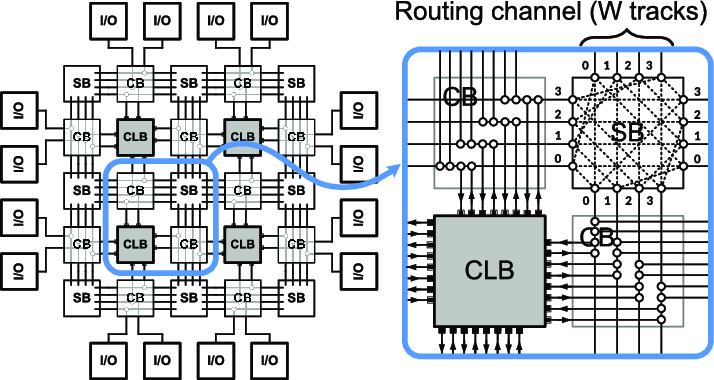
\includegraphics[height=2.6in]{figures/clb.png}
\caption{Generic FPGA hardware architecture. Depicted is the basic structure of a CLB and the interconnecting network.}
  \label{fig:clb}
\end{figure}

\pagebreak

Unlike general purpose systems such as CPUs or GPUs, this architecture allows the design of algorithms with arbitrary calculation widths, resulting in very good performance when processing images, both in power and time \ref{fig:op_watt}.

\begin{figure}[h!]
\centering
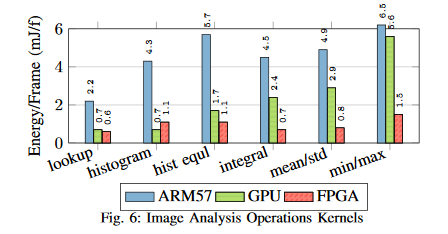
\includegraphics[height=1.8in]{figures/op_watt.png}
\caption{In image analysis kernels  such  as  lookuptable, histogram, and histogram equalization, the energy/frameconsumption  of  the  FPGA  achieves  an  average  reduction  of 1.2× compared  to  the  GPU.  For  kernels  with  more branching  conditions  and  complex  memory  access  patterns, such as integral image, mean/std, and min/max locations, the FPGA’s  implementation  achieved  an  average  reduction  ratioof 3.5× compared to the GPU\cite{ochoa-ruiz_high-level_2012}}
  \label{fig:op_watt}
\end{figure}

\pagebreak

The space environment not only limits avaible power, it also presents a challenge in the form of ionizing radiation. As this is one of the target markets for FPGA manufacturers, there are numerous chips with the necessary radiation resistance certifications.
%http://microelectronics.esa.int/techno/fpga_002_01-0-4.pdf
%https://amstel.estec.esa.int/tecedm/website/biblio/AFLDCIS2010.pdf
\\
ASICs provide the same design flexibility as FPGAs but their manufacturing rigidity allows them to achieve better performance by only including the specific design logic. However, their cost in small to medium scale projects is prohibitive. In addition, the flexibility of FPGAs allows reconfiguration already in the ship, allowing the use of different algorithms or bug fixes.
%https://iopscience.iop.org/article/10.1088/1742-6596/1195/1/012012/pdf
%https://amstel.estec.esa.int/tecedm/website/stag_ygt/Boada.pdf
\\
\\
In addition, since most algorithms share certain basic operations such as storage or high-precision arithmetic operations, FPGA manufacturers include certain prefabricated blocks in the circuit, which although remove some flexibility, provide better performance than the same logic in CLBs. These blocks are mainly RAM blocks and DSPs that allow a variety of operations, including multiplication or accumulation. This heterogeneous architecture \ref{fig:heterogenea} allows the implementation of high performance algorithms where it would be impossible using only logic and brings FPGAs a little closer to the scope of ASICs \cite{zhou_efficient_2013}.
\\
\begin{figure}[h!]
\centering
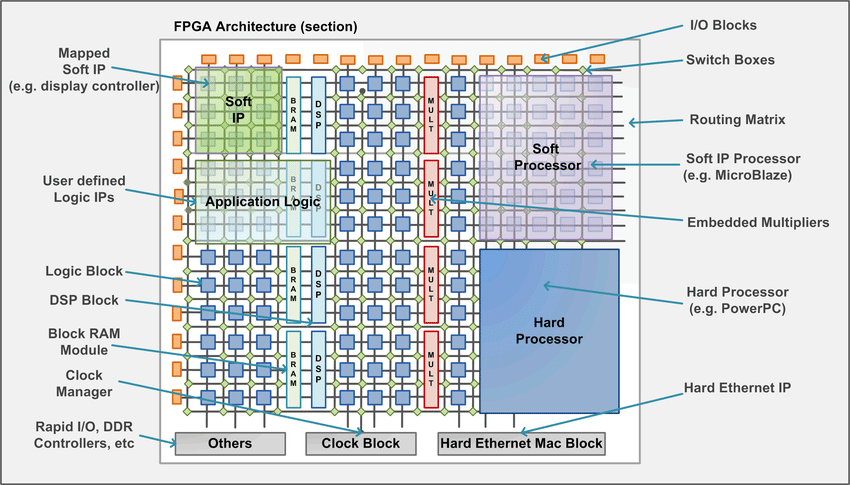
\includegraphics[height=2.5in]{figures/FPGA_heterogenea.png}
\caption{3: Heterogeneous FPGA platform, depicting general configurable resources, DSPs, BRAMs and soft (implemented in logic) and hard (prefabricated) CPUs}
  \label{fig:heterogenea}
\end{figure}
\\

\subsection{Hyperspectral imagery}
A standard camera captures images composed of 3 distinct light bands, which we humans perceive as red, green and blue. Their spectra correspond to high wavelengths between $564$ and $580 nm$ for red, mediums between $534$ and $545 nm$ for green and short ones between $420$ and $440 nm$ for blue. The rest of the spectra are invisible to our eyes.
\\
However, hyperspectral cameras capture information in many more spectra, both between the visible bands and outside them, allowing a much wider spectrum to be analyzed. These bands are usually shown as a third dimension, giving the name of hypercube to these images \ref{fig:cube}.
\\
\\
\begin{figure}[h!]
\centering
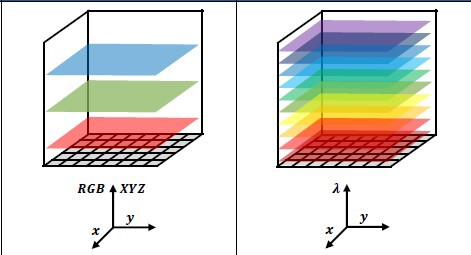
\includegraphics[height=2in]{figures/rgb_vs_hsi.jpeg}
\caption{Comparison between the three bands of a standard camera and the multiple bands of an hiperspectral camera}
  \label{fig:cube}
\end{figure}
\\
%url{https://towardsdatascience.com/what-are-hyper-spectral-images-a5de5d9fa91}
\\
\\
These spectra or bands form together an hyperspectral signature for each material, which when compared with aerial images allow the recognition of different types of vegetation, mineral deposits or contaminants on the earth's crust \ref{fig:cuprite}.
\\
\\
\begin{figure}[h!]
\centering
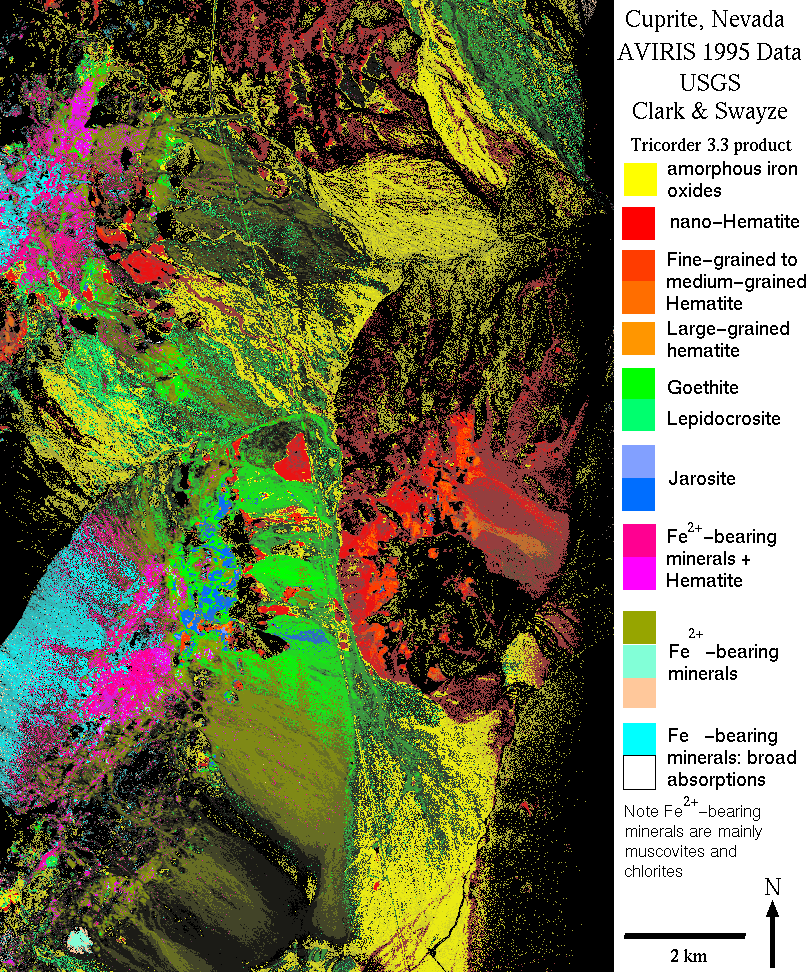
\includegraphics[height=6in]{figures/cuprite.png}
\caption{The map shown is a mineral map from an AVIRIS scene flown over Cuprite, Nevada, in 1995 \citep{noauthor_aviris_nodate}. It shows the mapping of many different minerals}
  \label{fig:cuprite}
\end{figure}
\clearpage


In this type of images we can talk about two types of resolutions: spatial and spectral, the latter being unique in this type of cameras. Spatial refers to the amount of meters covered by each pixel, so for the same camera you can change from one image to another. The spectral resolution refers to the separation between different wavelengths measured in a given range, that is, the more bands captured in a lower range, the higher the spectral resolution will be \cite{amigo_chapter_2020}.
\\

As technology advances, these resolutions continue to increase highlighting the need for commensurate processing systems.

\subsection{Anomaly detection}
In theory, a material should always have the same spectral signature. In practice, the captured signature will never be the same as the one measured in a laboratory because of differences in lighting, atmospheric effects, noise, etc. resulting in spectral variation for similar materials \cite{borsoi_spectral_2020}.

This has led to the development of algorithms that instead of classifying observations according to their signature, seek to classify the observations into unusual or anomalous materials and background. This assumes that the material -the target- is spectrally distinguishable from the background. The background is derived globally from the image assuming that it follows a normal distribution.

%\url{http://downloads.hindawi.com/journals/jece/2012/425947.pdf}\\
%\url{http://downloads.hindawi.com/journals/jece/2012/628479.pdf}\\
%\url{http://downloads.hindawi.com/journals/jece/2012/103286.pdf}\\
%\url{http://downloads.hindawi.com/journals/jece/2012/162106.pdf}

\subsubsection{RX algorithm}
The Reed-Xiaoli anomaly detector algorithm is a common algorithm that serves as the basis for many others.%\url{http://downloads.hindawi.com/journals/jece/2012/162106.pdf}\url{http://downloads.hindawi.com/journals/jece/2012/425947.pdf}\\%https://www.researchgate.net/publication/224166337_A_tutorial_overview_of_anomaly_detection_in_hyperspectral_images
%\url{http://downloads.hindawi.com/journals/jece/2012/162106.pdf}

The algorithm is defined by the following expression \cite{molero_fast_2011}:
\\
\[\delta ^{RX}(x) = (x-\mu)^{T}K^{-1}(x-\mu)\]

\paragraph{}
\phantomsection
\label{mayor}
Where $x$ is a hyperspectral pixel, a vector of size equal to the number of bands, $\mu$ is the mean of each band and $K$ is the covariance matrix. It is important to say that the results generated by the algorithm are grayscale 2D images. The anomalies have a high value, so the first anomaly corresponds to the pixel with the highest value, and so on.

\subsubsection{Other methods}
Apart from the RX algorithm, there are other methods for detecting anomalies, although a notable number of them are based on RX.

\subsubsection{Subspace methods}
Subspace methods are global and apply principal component analysis (PCA) or singular value decomposition (SVD) to the hypercube. The first PCA/SVD bands are supposed to be the background and are removed differently by each method. Not removing enough bands means that the anomalies can be lost in the background noise and removing too many would lead the anomalies to disappear. The determination of the correct number of bands to be removed is still under study \cite{borghys_hyperspectral_2012}.

\paragraph{Subspace RX}
In this method, the RX algorithm is applied to a limited number of PCA bands. The first components are discarded.

\paragraph{RX after orthogonal subspace projection}
In this method, the first PCA/SVD components define the subspace of the background and the data is projected onto an orthogonal space before applying XR.

\paragraph{RX after partialling out the clutter subspace}
In this method, clutter effect on a pixel is discarded component wise taking each of its spectral components as a linear combination of its high variance principal components. The RX algorithm is applied to the results.

\paragraph{Complimentary subspace detector}.
This algorithm is not based on RX. In CSD, the principal components with higher variance are used to define the subspace of the background and the other PCs to define the subspace of the target. The pixel is then projected onto the two subspaces and the result is the difference between them.

\subsubsection{Local methods}
In the local methods the background is derived from the neighboring pixels or surroundings of the pixel under test (PUT). Two windows are defined, a guard and an exterior, and the neighbors are the pixels that are between these two. Sometimes, for example in local RX, a third one is used where the covariance of the background is calculated in a window larger than the average of the background.

\paragraph{Quasi-local RX}
Quasi-local RX is a compromise between global RX and local RX, where the global covariance matrix is decomposed using eigenvector/eigenvalues. The eigenvectors are maintained, but the eigenvalues are replaced by the maximum local variance, resulting in lower detector scores in areas with high variance.

\begin{figure}[h!]
\centering
%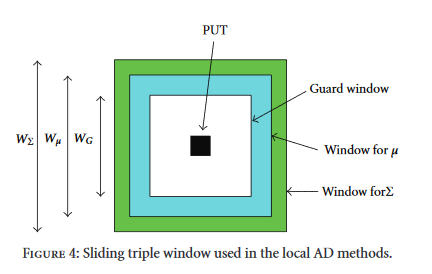
\includegraphics[height=2.5in]{figures/ventana.png}
\hspace*{100pt}%
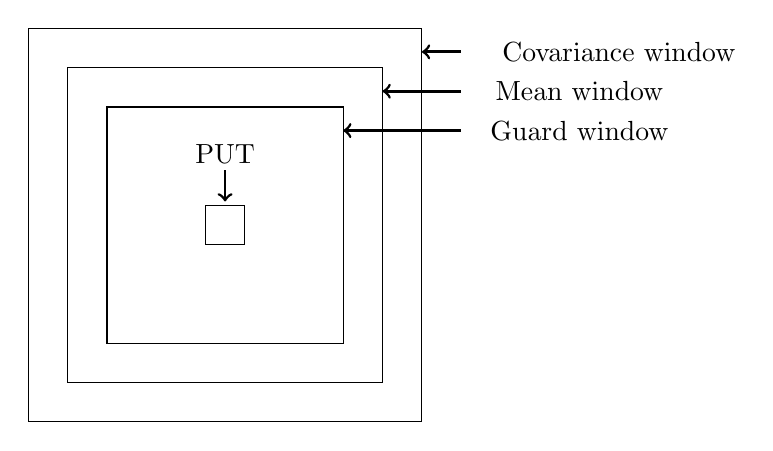
\begin{tikzpicture}
        \draw (0,0) rectangle (5,5);
        \draw[arrows=<-,line width=1pt](5,5-.3)--(5.5,5-.3);
        \draw (7.5,5-0.3) node{Covariance window};
        
        \draw (.5,.5) rectangle (4.5,4.5);
        \draw[arrows=<-,line width=1pt](4.5,4.5-.3)--(5.5,4.5-.3);
        \draw (7,4.5-0.3) node{Mean window};
        
        \draw (1,1) rectangle (4,4);
        \draw[arrows=<-,line width=1pt](4,4-.3)--(5.5,4-.3);
        \draw (7,4-0.3) node{Guard window};
        
        \draw (2.25,2.25) rectangle (2.75, 2.75);
        \draw[arrows=<-,line width=1pt](2.5, 3-.2)--(2.5, 3.2);
        \draw (2.5, 3.4) node{PUT};
    \end{tikzpicture}
\caption{Sliding triple window used in the local AD methods.}
  \label{fig:ventana}
\end{figure}

\subsubsection{Segmentation based methods}
In complex scenes it is difficult to assume that the background will be defined by a normal distribution, so methods have been developed to separate it into different classes.

\paragraph{Class-Conditional RX}
In this method the image is first segmented and the covariance and mean matrix calculated for each of these classes. Each pixel will correspond to the class in which its RX value is lower.

There are more methods within those based on segmentation, from those using stochastic functions such as Method Based on Multivariate Normal Mixture Models to methods based on Self-organizing maps.



\subsection{Comparing floating and fixed point}
\label{makereference}

In computer systems, there are two numerical representations for real numbers, fixed and floating point. They have different arithmetic, which gives them different range and resolution with the same number of bits. Therefore, there are certain applications or platforms more akin to one of them. For example, the ability of floating point numbers to contain in the same number of bits both very large and very small numbers and to adjust their resolution accordingly is very attractive from the programmer's point of view but the simplicity of fixed point operations allow their use in small microcontrollers or to save resources in FPGAs.%fuente
\begin{figure}[h!]
\centering
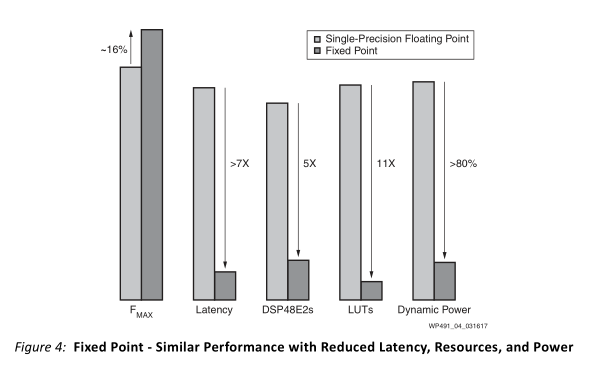
\includegraphics[height=2.5in]{figures/fp_vs_fp.png}
\caption{A FIR filter, originaly implemented as a single-precision floating-point filter and converted to fixed-point. The fixed-point design shows both resource reduction and latency improvements}
  \label{fig:fp}
\end{figure}
\\
Due to the high complexity of hyperspectral image analysis, current FPGAs have little capacity to implement some of these algorithms. Therefore, one of the objectives of this work is to perform two parallel implementations, one in floating point and another one in fixed point and compare their results.

\pagebreak
\section{Project plan}
First, an algorithm and a hardware platform are chosen. Desirably, this algorithm should be known and commonly found in the literature.
\\
This algorithm will be implemented in software and this implementation tested with real images against existing software such as ENVI or Spectral Python.
\\
The different algorithm stages will then be optimized for a hardware architecture and the transformation of the algorithm from floating point to integer or fixed point logic will be studied.
\\
This transformation requires design decisions that sacrifice precision with the goal of saving hardware resources, so the underlying hardware will have to be taken into account.
\\
Subsequently, a hardware validation of the design will be realized.
\\
Finally, a study will be carried out on the accuracy of the results obtained.
\\
\\
    \begin{figure}[h!]
    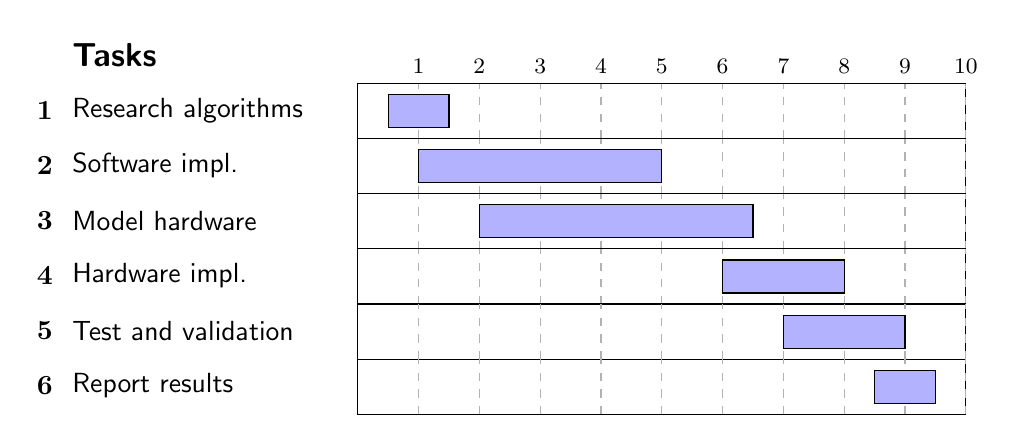
\begin{tikzpicture}
      \GanttHeader{\textwidth-0.6cm}{2ex}{3.5cm}{10}
      \Task{1}{Research algorithms}{0.5}{1}
      \Task{2}{Software impl.}{1}{4}
      \Task{3}{Model hardware}{2}{4.5}
      \Task{4}{Hardware impl.}{6}{2}
      \Task{5}{Test and validation}{7}{2}
      \Task{6}{Report results}{8.5}{1}

      %\arrowwhereboxesoverlap[thick,red,->]{1}{2}
      %\draw [blue,dashed,very thick,->] (2b) -- ++ (0.2,0) |- (4a);
\end{tikzpicture}
    \caption{Gantt diagram with an overview of months and tasks}
    \label{fig:gantt}
    \end{figure}

\cleardoublepage
%https://www3.ntu.edu.sg/home/ehchua/programming/java/datarepresentation.html
\chapter{Software Model}
The RX algorithm has been chosen for this work because it is the benchmark for this kind of algorithms \cite{borghys_hyperspectral_2012}, \cite{rosario_semiparametric_2012}, \cite{matteoli_tutorial_2010} and many existing algorithms basing on RX in some manner.
\\
In order to become familiar with the algorithm and create a platform where tests can be easily performed, a software implementation has been made as a first step.
\\
The first step is to divide the algorithm into simpler operations:
\begin{itemize}
\item Calculate the mean, deviation and K covariance matrix of the image
\item Calculate $K^{-1}$ that is, the inverse of the covariance matrix
\item Calculate $\delta ^{RX}$ for each pixel in the image
\item Sort the results
\end{itemize}
\pagebreak
\subsection{Mean, deviation and covariancce matrix}
One of the bottlenecks in this type of FPGA-based systems is the input and output of data \cite{tang_multi-fpga_2014}. Since the calculations of mean, variance and covariance matrix need the original matrix -a cube- for this, it has been decided to calculate these in a CPU and transmit the results to the FPGA. In addition, the operations are relatively simple for a CPU. Next, the pseudocode of the three is presented.
\\
\algnewcommand{\LineComment}[1]{\State \(\triangleright\) #1}
\begin{algorithm}
  \caption{Pseudocode for the mean, deviation and covariance matrix}
  \begin{algorithmic}[1]
    \LineComment{$bands$ : number of bands in the image}
    \LineComment{$pixels$ : number of pixels in the image}
    \LineComment{$A$ : the image in the form of a 2D matrix with $pixels \times bands$}
    \LineComment{$^T$ is used to denote the transpose of a matrix}
    \Statex
    \Function{mean}{$A$}
      %\State{$mean[bands]$}
      \For{$i \gets 0 \textrm{ to } bands-1$}
      	\State{$sum \gets 0$}
      	\For{$j \gets 0 \textrm{ to } pixels-1$}
       		\State{$sum \gets sum + A[i][j]$}
      	\EndFor
      	\State{$mean[i] \gets sum/pixels$}
      \EndFor
      \Return{$mean$}
    \EndFunction
    
    \Statex
    
    \Function{deviation}{$A, mean$}
    
      \Return{$A^T - mean$} \Comment{This operation is a matrix subtraction}
    \EndFunction
    
    \Statex
    
    \Function{covariance}{$deviation$}
    
      \Return{$deviation^T * deviation / (pixels-1)$}
    \EndFunction
  \end{algorithmic}
\end{algorithm}

The covariance, a $band^2$ matrix is then transmitted to the FPGA to calculate its inverse.
\clearpage

\subsection{Inverse}
\subsubsection{Choosing the algorithm}
Before starting the implementation, several algorithms to perform the inverse have been studied.
\paragraph{QR Factorization\citep{alberto_oliveira_de_souza_junior_exploration_2020}:}
QR factorization breaks down the $A$ matrix into the product of two matrices $A = QR$, with $Q$ being an orthogonal matrix and $R$ a superior triangular matrix. With this triangular matrix it becomes easy to calculate the inverse. However, although QR factorization can be efficiently performed on a powerful matrix multiplication module or several modules that can be executed simultaneously, such as in a GPU, it does not take advantage of the capabilities provided by our system such as arbitrary width arithmetic units.
\paragraph{Gauss Jordan elimination method\cite{gonzalez_fpga_2016}:}
The Gauss Jordan method dictates that if we have a $A$ matrix that can be transformed into the identity matrix through elementary operations, these same operations transform the identity matrix into $A^{-1}$. Since it is possible to execute these elementary operations in an entire row at once and the operations between rows are independent, this method is easily parallelizable.
Therefore, this was the chosen method.
\\
\\
Generally speaking, the execution of the algorithm takes place in such a way that:
\begin{enumerate}
\item An identity matrix is generated
\item The same operations are performed on both matrices until the $A$ matrix is transformed into the identity matrix
\item The result is in the matrix generated in the first step
\end{enumerate}
\noindent As seen in the following pseudocode, these elementary operations are performed in 3 steps:
\\
\\
\begin{algorithm}
  \caption{Pseudocode of the Gauss Jordan method}
  \begin{algorithmic}[1]
    %\Require{$A$ is a square matrix with the size $n*n$}
    \State{$A$ : a square matrix with the size $n*n$}
    \State{$A^{-1}$ : an identity matrix with the size $n*n$}
    \Statex
    \Function{inverse}{$A$}
      \For{$i \gets 0 \textrm{ to } n-1$} \Comment{Forward elimination to build the upper trangular matrix}
      \LineComment{row $i$ acts as the pivot}
      \If{$A[i][i] = 0$}   \Comment{If the later divisor is 0}
      	\For{$j \gets i+1 \textrm{ to } n-1$}
      		\If{$A[i][j] \neq 0$}
       			\State{$A[i] \gets A[j],\ A[j] \gets A[i]$}
      		\EndIf
      	\EndFor
      \EndIf
      \For{$j \gets 0 \textrm{ to } n-1$}
        \State{$A^{-1}[j] \gets A^{-1}[j]-A^{-1}[i]*(A[j][i]/A[i][i])$}
        \State{$A[j] \gets A[j]-A[i]*(A[j][i]/A[i][i])$}
        \Comment{These two operations may run in parallel}
      \EndFor
      \LineComment{After a complete iteration of the outer loop, the pivot contains the desired form}
      \EndFor
      \\
      \\
      \For{$i \gets n-1 \textrm{ to } 0$} \Comment{Backward elimination to build a diagonal matrix}
      \For{$j \gets i-1 \textrm{ to } 0$}
        \State{$A^{-1}[j] \gets A^{-1}[j]-A^{-1}[i]*(A[j][i]/A[i][i])$}
        \State{$A[j] \gets A[j]-A[i]*(A[j][i]/A[i][i])$}
        \Comment{These two operations may run in parallel}
      \EndFor
      \EndFor
      \\
      \\
      \For{$i \gets 0 \textrm{ to } n-1$} \Comment{Last division to build identity matrix}
        \State{$A^{-1}[i] \gets A^{-1}[i]*(1/A[i][i])$}
        \State{$A[i] \gets A[i]*(1/A[i][i])$}
        \LineComment{There is no need to update the values in the starting matrix}
      \EndFor
      \Return{$A^{-1}$}
    \EndFunction
  \end{algorithmic}
\end{algorithm}

It is also possible to calculate the inverse directly for each row, performing the three steps consecutievly in a row, but this way limits the parallelization between different rows.

\clearpage

\subsection{Matrix multiplication}
With the inverse of the convariance matrix calculated in the FPGA, the real RX algorithm can continue to be performed, where a hyperspectral pixel is multiplied with this inverse. This calculation will require the CPU to transmit the original image, the original image next to the average, or the deviation already calculated to the FPGA.
\\
\noindent The RX algorithm dictates that:
\[ rx(x) = (x-\mu)^{T} K^{-1}_{N \times N} (x-\mu) \]


\indent \(K^{-1}_{N \times N}\) \ \ \ being the inverse matrix with a dimension of \(N \times N\),\\
\indent \((x-\mu)\) \ \	being the deviation of a pixel a dimension of \(N \times 1\) and \\			
\indent \((x-\mu)^{T}\) \ it's transpose, with a dimension of \(1 \times N\).\\

\noindent In this step, the inverse matrix gets effectively multiplied by a unique pixel across all bands. Through row reduction, a single value for this pixel is recovered which can then be mapped to a 2d image.\\

Since the operands are heterogeneous, use can be made of the associative law on matrix products that dictates that:
	\[A * (B * C) = (A * B) * C\]
	to optimize the operation.\\


\paragraph{}
\phantomsection
\label{alternativa}
In the implementation sectiona study on what alternative to use will be carried out, as this depends heavily on the hardware architecture.

\section{Adapting the arithmetic}
As shown before in \autoref{fig:fp}, floating point arithmetic operations are very inefficient compared to fixed point operations. In the next chapter a transformation strategy will be defined and the steps followed to make this transition will be shown.
\\
\\
Taking advantage that the RX algorithm only needs relative and not exact values, ie, the highest value found in the results will be the most anomalous -see \ref{mayor}- regardless of whether it exceeds a certain threshold or not, the fixed-point representation may be simplified by ignoring the fractional part and keeping only the integer.

\subsection{DSP Blocks}
The DSP blocks are prefabricated circuits found next to the FPGA logic and implement arithmetic operations. These blocks allow to perform operations more efficiently and operate at higher frequencies than equivalent logic in the fabric, besides not occupying space in it. However, as they are prefabricated blocks, they do not offer the same flexibility as the rest of the FPGA logic. This implies that the size of the operands and the cost of operation resources will not always be proportionally related. Therefore, different widths have been tested and their resource usage has been noted. The results of these tests for multiplication are in the following table:

\begin{center}
 \begin{tabular}{|c c |c|} 
 \hline
 Width operand A & Width operand B & DSP48 Slices used \\ [0.5ex] 
 \hline\hline
 25 & 18 & 1 \\ 
 \hline
 35 & 25 & 2 \\
 \hline
 52 & 24 & 3 \\
 \hline
 42 & 35 & 4 \\
 \hline
 64 & 25 & 4 \\
 \hline
 52 & 42 & 6 \\
 \hline
\end{tabular}
\end{center}
Depending on the width of the operands, the operation will use a different amount of resources (data obtained for signed multiplication in Vivado 2019.2 on Xilinx Series 7 plates)
\\
\\
For subtraction operations up to 48bits, only one DSP is used, so they are not expected to require more than one block.
\\
The divisions cannot be implemented by this type of blocks, so they will use standard logic and can be used with an arbitrary width.
\\
\\
With this data for all the operations that are going to be carried out in the FPGA is recorded.
\\
\\
A hardware model implemented in software was used to determine the width of the multiplications. This model truncates both the input and output operands of each operation. The final results correspond then to the ratio of anomalies that are between the first x, up to 30.
\begin{figure}[h!]
\centering
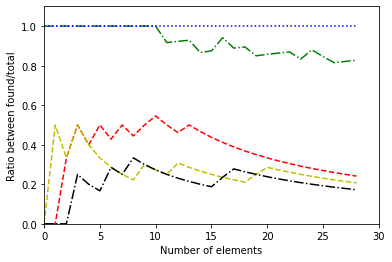
\includegraphics[height=2.5in]{figures/width.png}
\caption{Ratio of anomalies found in the first x using different bit widths for the multiplication. Dataset: Hydice}
  \label{fig:width}
\end{figure}

Como se puede observar en \autoref{fig:width}, ESTO TENGO QUE REPETIRLO.
\\

\subsection{Improving accuracy}
It is also necessary to create rules to shift the results to maintain the highest possible accuracy without producing overflow.
\\
For example, the divisions made in the inverse calculation produce very small numbers where the fractional part is relevant to the final result. Since this part is lost in integer arithmetic, it is necessary to multiply the operands to produce results where the point is shifted to the left. These multiplications will always be done in powers of 2, negative if required to decrease the bit width, as they are trivial to implement in an FPGA and do not require resources.
\\
\\
The results indicated that the greatest loss of accuracy occurred in the inverse calculation. Therefore, the model was revised and shifts were included in the initial matrix capture, in the initialization in the case of $A^{-1}$ and in the transfer to the FPGA in the case of $A$. Different shifts were also included for each phase of the inverse.



% +--------------------------------------------------------------------+
% | Sample Chapter 3
% +--------------------------------------------------------------------+

\cleardoublepage

% +--------------------------------------------------------------------+
% | Replace "This is Chapter 3" below with the title of your chapter.
% | LaTeX will automatically number the chapters.
% +--------------------------------------------------------------------+
    %\renewcommand{\chaptername}{Part}
    %\renewcommand{\thechapter}{}
\chapter{Implementation}
\label{makereference}

\section{General overview of the system}
La cámara proporciona los pixeles de la imagen por bandas. Las primeras operaciones a realizar con estos datos son calcular la media, con ella la deviación y con esta la covarianza. Dadas la relativa simpleza de estas operaciones pero sus altos requisitos en memoria, estas tres operaciones son realizadas en una CPU y sus resultados enviados a la FPGA. La FPGA comenzará el cálculo de las operaciones posteriores solo cuando tenga los resultados completos de la covarianza.
Los datos calculados por la CPU son introducidos en la FPGA a traves de FIFOs.
La FPGA calculará entonces la inversa de la matriz. Mientras tanto la CPU tendrá que escribir las medias calculadas y los valores que había recibido anteriormente de la cámara, uno por uno. Cuando termine la inversa, la FPGA realizará las dos últimas multiplicaciones de matrices y guardará los datos resultantes. Con el ultimo pixel procesado, la FPGA escribirá las anomalías ordenadas de mayor a menor en otra FIFO para ser leída por la CPU.
\\
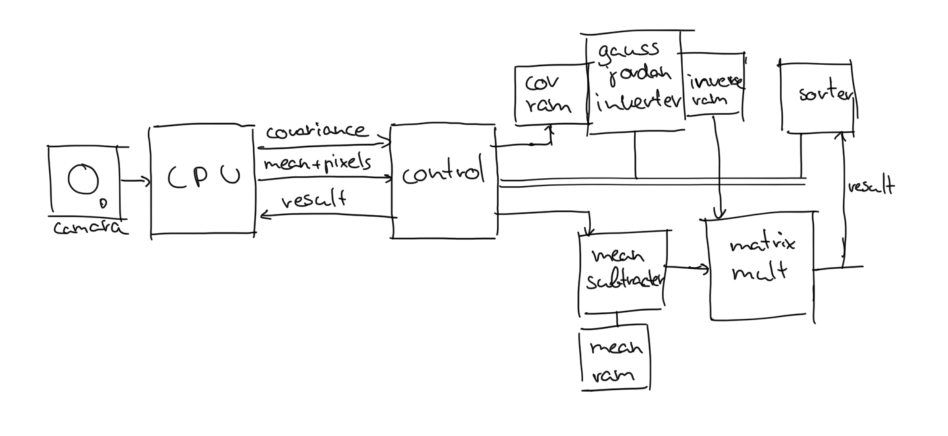
\includegraphics[height=3.5in]{figures/bus.png}


\section{Description by module}
\section{Control}
Este modulo actúa sobre los módulos inferiores, tanto para controlar el traspaso de datos entre ellos como para arbitrar el acceso a las RAMS y las FIFOs que comunican con la CPU.

Cabe mencionar que también realiza ciertas comprobaciones en la escritura de la covarianza para asegurar que la primera división de la inversa no se realiza con un 0, es decir, que la posición (0, 0) en la matriz de covarianzas es /= 0.
\\
\\
AQUÍ TENGO LA ELECCIÓN DE PONER UN DIAGRAMA DE ESTADOS, PSEUDOCÓDIGO O DEJARLO VACÍO
\\
\\

\section{Inverter}
La inversa es con diferencia el módulo más complejo y con más gasto de recursos. Además, el estudio realizado en software ha mostrado que es con diferencia el paso más susceptible a empeorar la precisión de los resultados finales. Por estas razones se ha hecho especial hincapié en su diseño.
\\
\subsection{Choosing the algorithm}
Antes de empezar la implementación se han estudiado varios algoritmos para realizar la inversa.
\\
\\
\textbf{QR decomposition:}
\\
La decomposición QR descompone la matriz $A$ en el producto de dos matrices $A = QR$, siendo $Q$ una matriz ortogonal y $R$ una matriz triangular superior. Con esta matriz triangular resulta sencillo calcular la inversa. Sin embargo, aunque la decomposición QR puede ser beneficiosa mientras que se cuente con un modulo de multiplicación matricial potente o varios módulos que puedan ser ejecutados de forma simultanea, como puede ser en una GPU, no aprovecha las ventajas proporcionadas por nuestro sistema como pueden ser un tamaño de matrices determinado.
\\
\\
\textbf{Gauss Jordan elimination method:}
\\
El método de Gauss Jordan dicta que si tenemos una matriz $A$ que puede ser transformada en la matriz identidad a través de operaciones elementales, estas mismas operaciones tranforman la matriz identidad en $A^{-1}$. Puesto que es posible ejecutar estas operaciones elementales en una fila entera y las operaciones entre filas son independientes, este método es fácilmente paralelizable.
Por tanto, este fue el método elegido.
\\
A rasgos generales, la ejecución del algoritmo transcurre tal que:
\begin{enumerate}
\item Se genera una matriz identidad
\item Se realizan las mismas operaciones sobre ambas matrices hasta transformar la matriz $A$ en la matriz identidad
\item El resultado se encuentra en la matriz generada en el primer paso
\end{enumerate}

Estas operaciones elementales se realizan en 3 pasos, primero se transforma la matriz A en forma con triangulo superior, luego se resuelve el triangulo inferior para transformarla en diagonal y finalmente se divide la matriz entre si misma hasta conseguir la forma escalonada reducida por filas. (row canonical form)
\\
\\
\algnewcommand{\LineComment}[1]{\State \(\triangleright\) #1}
\begin{algorithm}
  \caption{Pseudocode of the Gauss Jordan method}
  \begin{algorithmic}[1]
    \Require{$A$ is a square matrix with the size $n*n$}
    \Statex
    \Function{inverse}{$A$}
      \For{$i \gets 0 \textrm{ to } n-1$} \Comment{Forward elimination to build the upper trangular matrix}
      \LineComment{row $i$ acts as the pivot}
      \If{$A[i][i] = 0$}   \Comment{If the later divisor is 0}
      	\For{$j \gets 0 \textrm{ to } n-1$}
      		\If{$A[i][j] \neq 0$}
       			\State{$A[i] \gets A[j], A[j] \gets A[i]$}
      		\EndIf
      	\EndFor
      \EndIf
      \For{$j \gets 0 \textrm{ to } n-1$}
        \State{$A^{-1}[j] \gets A^{-1}[j]-^{-1}A[i]*A[j][i]/A[i][i]$}
        \State{$A[j] \gets A[j]-A[i]*A[j][i]/A[i][i]$}
        \Comment{These two operations may run in parallel}
      \EndFor
      \LineComment{After a complete iteration of the outer loop, row $i$ contains the desired form}
      \EndFor
    \EndFunction
  \end{algorithmic}
\end{algorithm}

AQUI TENGO QUE PONER LOS OTROS PASOS DEL ALGORITMO
\\
\\
\\
También es posible calcular la inversa directamente para cada fila, realizando los 3 pasos seguidos, pero esta forma limita la paralelización entre diferentes filas.
\\
\\
\\

\subsection{Optimizaciones del algoritmo de cara a hardware}
Las operaciones a realizar en los tres pasos - triangulo, superior y diagonal- son similares, así que con el fin de ahorrar recursos se han implementado sobre la misma lógica. Existe un proceso superior con los contadores para controlar el orden de su ejecución. (counterproc). En el caso de la diagonal, se ha creado un cortociircuito para evitar el calculo de la resta.
\\
\\
Debería poner un dibujito con todos los procesos
\\
\\
Para mejorar el rendimiento del módulo, las operaciones sobre la matriz A y la matriz I se ejecutan de forma simultanea. Además, mientras las operaciones de una fila se encuentran procesándose, las siguientes filas son procesadas. La unica espera ocurre cuando se necesita el resultado de una fila para el procesado de las siguientes. Esto es similar a loop unrolling. Para ello, se usan varios procesos para controlar la lectura, la escritura y la captura de la fila que actua como pivote (writeproc y captureiproc). 
\\
\\
Debería poner una rueda con colores con los calculos que están el pipeline, los encolados, etc
\\
\\
Como se puede observar en el algoritmo, la fila [j] es usada dos veces.
\[A^{-1}[j] \gets A^{-1}[j]-^{-1}A[i]*A[j][i]/A[i][i]\]
Aqui poner colores
Para poder realizar operaciones sobre filas posteriores sin retrasar lecturas, es necesario guardar este dato en una memoria auxiliar y leerlo en el momento en el que se vuelva a necesitar. Esta memoria está construida a partir de una fifo tempconvj.
\\
\\
Además, se puede observar que el algoritmo exige una comprobación en la fila pivote y un posible trueque de filas. Esto es necesario ya que este valor es posteriormente el dividendo, por lo que un 0 provocaría un fallo en el cálculo.
-> Recibir fila i
-> Escribir fila i en posicion i
-> Recibir fila i+1 (nuevo pivote)
-> Si la fila no contiene un 0 en la posicion i+1, escribir en i+1 y escribir siguiente filas normalmente
-> Si la fila contiene un 0 en la posicion i+1, escribir en i+2
-> Recibir fila i+2
-> Si la fila no contiene un 0 en la posicion i+1, escribir en i+1 y escribir filas a partir de la i+2
-> Si la fila contiene un 0 en la posicion i+1, escribi...
joder debo hacer un algoritmo en pseudocodigo



Al aprovechar las escrituras para realizar estas comprobaciones, se evita el tener que leer filas de forma innecesaria y la latencia que ello conllevaría.

Además, puesto que las memorias RAM requieren de un par de ciclos de latencia para lectura y escritura, 2 y 3 respectivamente, los treques de filas se realizan a través de una tabla de renonbrado. Esta tabla es local, por lo que los resultados tienen que ser reordenados antes de salir del modulo. Puesto que estos trueques solo ocurren en el calculo del triangulo superior, se puede aprovechar el triangulo inferior para reordenarlos. El sistema de reordenamiento es muy simple, los datos entran en el pipeline en el orden en el que se han procesado en el paso anterior y son escritos en su orden natural. Esto implica que los resultados de este reordenamiento van a ser correctos siempre y cuando ambas filas que necesiten ser rotadas se encuentren en el pipeline de procesamiento, que en el caso de  punto fijo tiene aproximandamente un tamaño de 80. Resultados experimentales muestran que rara vez hay que rotar filas (aunque lo suficiente como para ser recomendable la inclusión de un metodo que lidie con ello), pero que estas rotaciones rara vez exceden más una o dos posiciones en adelante.
\\
\\
En la transformación a aritmética de punto fijo se descubrió que el cálculo de la inversa es que más error llega a introducir en los resultados finales del algoritmo, por lo tanto se ha hecho estudio exhaustivo en  sobre como minimizarlo. Con la tabla de uso de los dsp [referirse a la tabla mencionada anteriormente], se ha intentado encontrar el mejor balance entre DSP y menor error introducido en la operación.
Para poder aprovechar este balance, ha sido necesario reducir los valores en los que la precision limitada producía desbordamientos y aumentar valores pequeños para otorgarles más peso en las operaciones. Además, al realizar las operaciones de generación de identidad, triangulo superior, inferior y diagonal de forma independiente, se ha podido colocar diferentes desplazamientos y afinar todavía más la resolucion del algoritmo. Estas operaciones se encuentran en el proceso (shiftproc)
\\
\\
Tabla con los resultados con todo en 1, con la generacion de identidad en 29, y con todo metido. 
\\
\\
Por ultimo, cabe decir que existe un error en la generación de divisores de Xilinx. Cuando se introducen números cerca del limite de precision se pierde el control del signo. Por lo tanto se ha colocado un modulo antes de la división que convierte todos los operandos introducidos en positivos y guarda su posición en el pipeline. En el momento de producirse los resultados, se comprueba el tag en el pipeline, se calcula el negativo y se sustituye si es necesario. El proceso es divisorproc.

\section{Mean subtract}
El modulo de mean subtract simplemente realiza la resta de la media a la matriz de pixeles original. Este calculo es la deviacion. Aunque ya había sido calculada por la cpu, merece la pena implementarla en la fpga en el caso de que la cpu deba deshechar la deviacion por falta de memoria pero pueda volver a obtener la imagen original de la cámara. El calculo de la media si que se requiere puesto que su tamaño es mucho menor.
El modulo recibe los elementos desde el modulo superior. Los primeros que son la media son guardados en una ram que es tratada como un buffer circular, y los elementos que le siguen son restados directamente y devueltos al modulo superior de nuevo.


\section{Matrix multiplication}

N bandas\\
M pixeles\\
https://www.harrisgeospatial.com/docs/RXAnomalyDetection.html\\

\noindent This module performs the multiplication between the deviation and inverse matrixes.
\[ rx(x) = (x-\mu)^{T} K^{-1}_{N \times N} (x-\mu) \]


\indent \(K^{-1}_{N \times N}\) \ \ \ being the inverse matrix with a dimension of \(N \times N\),\\
\indent \((x-\mu)\) \ \	being the deviation of a pixel a dimension of \(N \times 1\) and \\			
\indent \((x-\mu)^{T}\) \ its transpose, with a dimension of \(1 \times N\).\\

The inverse gets read directly from the inverse module's output BRAM and the deviation matrix from two  FIFOS written by the CPU. The result gets written back to another FIFO.

In this step, the inverse matrix gets effectively multiplied by a unique pixel across all bands. Through row reduction, a single value for this pixel is recovered which can then be mapped to a 2d image.\\

Since the operands are heterogeneous, use is made of the associative law on matrix products that dictates that:
	\[A * (B * C) = (A * B) * C\]
	to optimize the operation.\\


\newcommand\rb{\colorbox{red!20}}
\newcommand\bb{\colorbox{blue!20}}
\newcommand\gb{\colorbox{green!20}}
\newcommand\rr{\rowcolor{red!20}}
\newcommand\br{\rowcolor{blue!20}}
\newcommand\gr{\rowcolor{green!20}}

\noindent Following will be a comparison of the first required multiplication in both methods:
\begin{quote}
	\((x-\mu)^{T} K^{-1}_{N \times N}\):	
	A row from the inverse and the whole column of the deviation get read, each element multiplied with its correspondent and all products added together. If stalls were to be avoided, this sum would need to be computed every cycle, which can easily be achieved with an adder tree.
\end{quote}

\begin{figure}[h]%t=top, b=bottom, h=here
\[
\begin{pmatrix}
\rr a & b & c \\ 
\br d & e & f \\ 
\gr g & h & i
\end{pmatrix}
*
\begin{pmatrix}
1\\
2\\
3
\end{pmatrix}
=
\begin{pmatrix}
\rr 1*a+2*b+3*c\\
\br 1*d+2*e+3*f\\
\gr 1*g+2*h+3*i
\end{pmatrix} 
\]
\caption[Optional: Short caption to appear in List of Figures]{First proposed method for the computation of a single pixel: red, blue and green represent data processed in the first, second and third cycles respectively. Note that the entire deviation data of that pixel gets used every cycle}
\end{figure}
\pagebreak
		
\begin{quote}
	\(K^{-1}_{N \times N} (x-\mu)\):
	The inverse gets also read row by row, but the deviation matrix only by elements. Each element of the first row of the matrix gets multiplied with the first element of the deviation, the result accumulated, and continued with the next pair row/element. This goes for \(N\) cycles, that is, a whole inverse matrix and a whole pixel in the deviation matrix. The result is \(N\) accumulated values which get flushed every \(N\) cycles, which ends up being the same throughput as the former method.
\end{quote}

\begin{figure}[h]%t=top, b=bottom, h=here
\[
\begin{pmatrix}
\rb1 & \bb 2 & \gb 3
\end{pmatrix}
*
\begin{pmatrix}
\rr a & b & c \\ 
\br d & e & f \\ 
\gr g & h & i
\end{pmatrix}
=
\begin{pmatrix}
\rb{1*a}+\bb{2*d}+\gb{3*g} & \rb{1*b}+\bb{2*e}+\gb{3*h} & \rb{1*c}+\bb{2*f}+\gb{3*i}
\end{pmatrix} 
\]
\caption[Optional: Short caption to appear in List of Figures]{Second proposed method: red, blue and green represent data processed in the first, second and third cycles respectively. Here only an element of the deviation data gets accessed each cycle.}
\end{figure}

While both methods have equivalent cost in time -the former has the added latency of the adder tree, the latter the latency of the accumulators- and also similar cost in DSP usage, data input by row is less taxing on the CPU and its FIFO structure can be reused for the second multiplication. Henceforth, the second approach was chosen.
\\

The second multiplication is similar in both steps, a \(1 \times N\) by \(N \times 1\) multiplication. One operand comes every cycle and each \(N\) cycles all products get added together. This sum is realized through an accumulator.\\

The module contains three subprocesses:
\begin{itemize}
	\item \emph{first\_mac} reads the inverse and performs its multiplication with the first FIFO. The products are then accumulated till a whole pixel has been computed.
	\item \emph{second\_mac} stores the results of \emph{first\_mac} in registers and performs the multiplication with the second FIFO, with the result being accumulated. Every cycle, the registers are shifted so a new multiplication is done.
	\item \emph{write\_proc} controls the writing of the results from \emph{second\_mac} to the result FIFO.
\end{itemize}



\section{sorter}
 El sorter recibe un valor y un par de coordenadas cada nbandas ciclos. Estos valores son escritos en una memoria ram que actua como una lista ordenada. Cada valor introducido es comparado con la cabeza de la lista, el valor más alto guardado y el otro es guardado en una variable temporal y comparada con el segundo valor en la lista, así sucesivamente. Puesto que se recibe un valor cada nbandas, el numero maximo de valores posibles a almacenar en esta lista es también nbandas. El resto de valores son deshechados. Cuando se ha introducido el ultimo valor, el modulo comunica los pixeles más altos, es decir, más anomalos, al modulo superior para que estos sean comunicados a la cpu.
\section{ejecucion paso a paso}
que tengo que poner aqui


\cleardoublepage
\chapter{Resultados}
%\label{ch:chapter1}
\label{makereference}
\section{plataforma reconfigurabke}

\begin{center}
 \begin{tabular}{|c|c|c|c|c|} 
 \hline
 Module & LUT & Register & BRAM & DSP \\ [0.5ex] 
 \hline\hline
 Inverse & 0 & 0 & 0 & 0\\ 
 \hline
 Mean subtraction & 0 & 0 & 0 & 0\\ 
 \hline
 Matrix multiplication & 0 & 0 & 0 & 0\\ 
 \hline
 Sort results & 0 & 0 & 0 & 0\\ 
 \hline
\end{tabular}
\end{center}

\begin{center}
 \begin{tabular}{|c|c|} 
 \hline
 Stage & Complexity \\ [0.5ex] 
 \hline\hline
 Inverse & $\mathcal{O}(bands+bands^2) = \mathcal{O}(bands^2)$\\ 
 \hline
 Mean subtraction & $\mathcal{O}(1)$\\
 \hline
 Matrix multiplication & $\mathcal{O}(bands*pixels+bands)$\\
 \hline
 Sort results & $\mathcal{O}(2*bands) = \mathcal{O}(bands)$\\
 \hline
\end{tabular}
\end{center}

\section{conjunto de images hiperespectrales}

Hydice: Bands 	210
Spectrum [nm] 	400-2500
Spat.Res. [m] 	0-0 
Aviris:
Spectral range: 360 - 2500 nm with a total of 224 bands. 
667*667 px
20m -> 12km
\section{evaluacion de las anomalias detectadas}
Aqui es donde dudo de si van los graficos anteriores que he puesto en la seccion de transformacion
\section{evaluacion del rendimiento}
\cleardoublepage
\chapter{Conclusions}
%\label{ch:chapter1}
\label{makereference}
Hyperspectral image processing is a very powerful tool that facilitates mining operations, target tracking or contamination analysis. The technological advances in these cameras accentuates the need to perform this type of analysis on board and with it the use of specific platforms such as FPGAs.
\\
\\
The complete analysis of this type of images is not always feasible and target detection algorithms such as the one presented here allow not only a significant reduction in bandwidth requirements but also allow the use of this type of sensors in real-time applications.
\\
\\
The results obtained are positive since they show a reduction in the use of resources and  compared to other previous implementations thanks to its approach through the use of fixed point logic. The use of a reconfigurable platform also allows the precision of this system to be adjusted even after it has been put into operation.
\\

% +-------------------------------------------------------------------------+
% | References                                                              |
% +-------------------------------------------------------------------------+

\bibliography{references}
%\bibliographystyle{ieeetr}

% +--------------------------------------------------------------------+
% | Finally, we generate the appendix.  To add or delete appendices,
% | add or remove the line
% |
% |     \input{appendixX.tex}
% |
% | where "X" is the letter designation of the Appendix (A, B, C, etc.)
% | You should have one \input{appendixX.tex} line and a corresponding
% | file appendixX.tex for each appendix.                                 |
% +--------------------------------------------------------------------+

\appendix
%\input{appendixA.tex}
%\input{appendixB.tex}

\end{document}
